\documentclass[10pt]{article}
\usepackage[margin=1.5in]{geometry}
\usepackage[strict]{changepage}
\usepackage{threeparttable, adjustbox, tabularx, longtable}
\usepackage{amsmath, amssymb, amsthm}
\usepackage{hyperref, achicago}
\usepackage{caption, graphicx}
\usepackage{secdot, sectsty}
\usepackage{booktabs}
\usepackage{pdflscape}
\usepackage{placeins}
\usepackage{setspace}
\usepackage{xcolor}

\allsectionsfont{\rmfamily}
\sectionfont{\normalsize}
\subsectionfont{\normalfont\normalsize\selectfont\itshape}
\subsubsectionfont{\normalfont\normalsize\selectfont\itshape}

\sectiondot{subsection}

\renewcommand\thesection{\Roman{section}}
\renewcommand\thesubsection{\Alph{subsection}}

\makeatletter
\newcommand*{\centerfloat}{\parindent \z@ \leftskip \z@ \@plus 1fil \@minus \textwidth \rightskip \leftskip \parfillskip \z@skip}
\makeatother

\newcommand{\specialcell}[2][c]{\begin{tabular}[#1]{@{}c@{}}#2\end{tabular}}

\begin{document}

\onehalfspacing

\title{Using Lotteries to Encourage Saving: Experimental Evidence from Kenya}

\author{Justin Abraham\thanks{Department of Psychology, Princeton University. \protect\href{mailto:justinra@princeton.edu}{justinra@princeton.edu}}, Merve Akbas\thanks{Department of Economics, Duke University. \protect\href{mailto:merve.akbas@duke.edu}{merve.akbas@duke.edu}}, Dan Ariely\thanks{Fuqua School of Business, Duke University. \protect\href{mailto:dan@danariely.com}{dan@danariely.com}}, and Chaning Jang\thanks{Department of Psychology, Princeton University and The Busara Center for Behavioral Economics. \protect\href{mailto:cjang@princeton.edu}{cjang@princeton.edu}}}

\maketitle

\begin{abstract}
This paper reports a ``lab-in-the-field'' experiment that test a savings scheme incorporating lottery-like payoffs to traditional savings accounts. We provide a mobile savings product to 311 informal residents in Nairobi, Kenya and observe account activity over a 60-day period. We find that respondents with lottery-linked deposit accounts (LLDAs) made 30-40\% more deposits on average over the project period than respondents receiving a matched incentive. Moreover, this increase in account activity is due to respondents making more deposits per day and depositing for more days. We also show that when presented with potential winnings from previous days, respondents with LLDAs increased self-reported gambling activity by 15\%. Our results suggest that LLDAs are a promising tool to improve savings among the poor but that product design has considerable implications on gambling behavior.
\end{abstract}

\newpage

\section{Introduction}

	Although access to savings accounts for the poor has improved in recent years, demand for and usage of savings accounts remains a stumbling block hindering full financial inclusion \shortcite{kendall_measuring_2010}. Standard interventions have focused on lowering transaction costs, boosting incentives to save, and improving financial infrastructure in underserved areas \shortcite{ashraf_deposit_2006,schreiner_match_2006,allen_improving_2014}. The growth of mobile money services has been especially important in encouraging the use of savings account in Sub-Saharan Africa \shortcite{demirguc-kunt_global_2015}. A recent focus on behavioral barriers to saving has been fruitful. Behaviorally-informed product designs, including SMS reminders \shortcite{karlan_getting_2010}, commitment devices \shortcite{ashraf_tying_2006,dupas_why_2013}, default contributions \shortcite{thaler_save_2004,chetty_active_2014}, and tokens \shortcite{akbas_how_2016}, have been shown to be extremely cost-effective compared to traditional economic interventions.
	
	Our study focuses on an alternative scheme that incorporates lottery-like payoffs to traditional savings accounts. Lottery-linked deposit accounts (LLDAs) have been in use since at least the 17\textsuperscript{th} century and presently exist in various forms around the globe \shortcite{murphy_lotteries_2005,kearney_making_2010}. NS\&I Premium Bonds in the U.K. and First National Bank's ``A-Million-A-Month'' Account in South Africa are two prominent examples of this type of savings product. Lottery-linked savings accounts are unique in that they provide stochastic returns as a function of savings or deposits. Savers will forego interest for a probabilistic payoff but face no risk of losing their principal. This unique feature makes the product attractive as a tool to promote financial inclusion. Lottery expenditures as a proportion of income are highest among the poor, which suggests that they may be especially responsive to lottery-like incentive structures \shortcite{brown_socio-economic_1992}. Furthermore, there is some evidence that usage of lottery-linked accounts displaces regular gambling behavior, thereby redirecting gambling expenditures into savings \shortcite{cookson_when_2016}.

	How might lotteries induce savings? Extensions of von Neumann-Morgenstern expected utility can explain why risk-averse individuals might prefer stochastic over fixed returns. These include the over-weighting of small probabilities \shortcite{kahneman_prospect_1979}, preferences for skewness \shortcite{golec_bettors_1998}, excitement from gambling \shortcite{conlisk_utility_1993}, or consumption indivisibilities faced by poor households \shortcite{mccaffrey_why_1994}. Persistent gambling behavior in the face of losses might also stem from cognitive biases such as the gambler's fallacy and the ``hot hand'' fallacy \shortcite{gilovich_hot_1985}. There also exists evidence that aversion to anticipated regret could drive gambling behavior \shortcite{zeelenberg_consequences_2004}.

	Literature on the potential demand for LLDAs is extensive, but empirical evidence as to its effect on savings behavior is scarce. Two recent experimental studies provide support for an extant benefit of stochastic returns on saving for the future. \shortciteN{atalay_savings_2014} conducted an online portfolio-choice experiment that resulted in respondents saving an additional 12 percentage points more with lottery-linked and regular savings than with regular savings alone. Notably, respondents who saw an increase in total savings shifted away from lottery expenditures and consumption rather than from regular savings. \shortciteN{filiz-ozbay_lottery_2015} found respondents are more likely to delay payments with lottery-like returns compared to guaranteed interest of equivalent expected value. This finding suggests that lottery-linked schemes can be designed to be revenue neutral in expectation for account providers while still promoting savings. \shortciteN{filiz-ozbay_lottery_2015} additionally estimate structural parameters and argue that probability weights better explain the result than individual preferences for skewness. Outside the laboratory, evidence regarding LLDAs is much more limited and diverges from experimental findings. \shortciteN{loibl_testing_2016} conducted a randomized evaluation of Individual Development Accounts (IDAs) in the U.S. that incorporated a lottery-based savings match. That study found no significant effect of the program relative to guaranteed matching, even when it was bundled with reminder calls and frequent deposit deadlines. They attribute the result to liquidity constraints among their sample, which potentially precluded the benefits of behavioral interventions. Research on the effect of other lottery-based incentive schemes relative to deterministic incentives remains inconclusive \shortcite{halpern_lottery-based_2011,gajic_cost-effectiveness_2011,brune_effect_2015}.

	The present study is a ``lab-in-the-field'' experiment testing the effects of lottery-linked savings on savings behavior. We provide a mobile savings product to 311 informal residents in Nairobi, Kenya and observe account activity over a 60-day period. We minimize barriers to saving by utilizing Safaricom's \textit{Sambaza} mobile savings technology. This platform also allows us to collect detailed data on participant transactions to be able to examine savings behavior over time. One group is randomly assigned a savings account which provides a fixed 5\% match to all deposits. A second group is assigned an account that yields stochastic returns, equal in expectation to the 5\% match, through a lottery conducted on a daily basis. For each day a respondent makes a non-zero deposit, they receive a lottery ticket and an opportunity to win a prize instead of the fixed match. We compare the interest and lottery groups to determine how LLDAs impact savings behavior. A third group is given the same lottery-linked account with the additional feature that respondents receive a lottery ticket every day regardless of saving but cannot claim the prize untile after making a deposit. The key feature of this ``regret'' treatment is that respondents observe the lottery results and potential prize at the end of each day. We test this treatment aginst the lottery treatment to determine whether experienced regret from being unable to claim a prize affects decisions to save.

	We find that respondents with LLDAs made 30-40\% more deposits on average over the project period than respondents receiving the matched incentive. Moreover, this increase in account activity is due to respondents making more deposits per day and depositing over more days during the savingss period. Respondents saved 50\% more per day and saved 5 days more compared to the control group. Effects on the number of deposits were more acute for respondents who are female, who are over 30 years old, with lower incomes, who are less prone to gambling, and who are risk-seeking, though we report no significant heterogeneous effects. There were no significant differences in effects on saving between the regular LLDA and the LLDA with regret framing. Interestingly, we find no effect of LLDAs on total amount saved or on the size of each deposit. Respondents made smaller, more frequent deposits compared to the control group. We find no evidence of the LLDA displacing savings from other sources. On gambling behavior, we find that 27\% respondents in the regret framing self-report higher gambling activity compared to 12\% in the control group.

	This study contributes to the literature as one of the first randomized evaluations examining the impact of LLDAs on real-world savings behavior. Moreover, the study's unique experimental design allows us to identify dynamic effects -- respondents make more frequent deposits to their accounts when given lottery-based returns. This result suggests that the appeal of gambling may be enough to induce a change in savings behavior. LLDAs may thus improve utilization among existing account holders and be able to attract new savers to open formal savings accounts. Frequent deposits may also have long-term benefits by encouraging the formation of a savings habit \shortcite{alessie_saving_2009}. From a policy perspective, LLDAs are appealing because they are more effective at changing savings behavior than matched incentives without an increase in the incentive itself. However, LLDAs may not be revenue neutral if financial institutions incur greater transaction costs as a result of more frequent deposits.

	Our study also shows that respondents with LLDAs with regret framing increased self-reported gambling activity relative to the control group. If LLDAs contribute to problem gambling, the program is potentially welfare-decreasing for poor households already susceptible to costly gambling behavior. \shortciteN{cookson_when_2016} reports a 50\% reduction of casino gambling in Nebraska as a result of enrollment in an LLDA bundled with an anti-gambling advertising campaign. The difference from our results suggests that additional program components could diminish effects on outside gambling. Overall, we document several advantages of LLDAs over fixed-incentive schemes when it comes to promoting financial inclusion and show that product design is crucial in moderating adverse effects on gambling behavior.

	The remainder of the paper is structured as follows. Section \ref{sec:design} describes our experimental design, Section \ref{sec:est} outlines our estimation strategy, and Section \ref{sec:results} displays our main results.

% 	Talk about results

% 		Effect on no. of deposits though no effect on total saved
% 		Improves the streak of consecutive savings
% 		Important in possibly encouraging habit-formation
% 		Het effects on savings: no prior savings for deposits, female, single households for regret, older, educated, actual savings for educated, low income, low prior gambling, unemployed for regret, risk averse
% 		Het effects on gambling: male, single for regret, educated for regret, prior gambling, unemployed
% 		Trasaction-level dynamics: check whether habit formation varies across treatment groups
% 		Misc: No effect on actual savings, increase in self-reported gambling behavior like \shortcite{brown_socio-economic_1992} \shortciteN{shawn_allen_cole_can_2014} \shortcite{maynard_consumer_2008}

% 	Talk about contributions (how it solves shortcomings discussed in previous research)

% 		Focus on a potentially important outcome (no. of deposits/streak) determining long-term savings behavior previously neglected in the literature
% 		\textcolor{red}{Could briefly discuss links to habit-formation literature}
% 		Less than 20\% of banked adults in Sub-Saharan Africa make more than 2 deposits in a month \shortcite{demirguc-kunt_global_2015}
% 		Examine dynamic savings behavior rather than one-shot \shortcite{brune_effect_2015} 
% 		Lab-in-the-field allows joint investigation of parametrics in a natural setting

% 	Talk about policy implications

% \section{Theoretical Framework}

% 	Why might this work? over-weighting of small probabilities \shortcite{kahneman_prospect_1979}, preferences for skewness \shortcite{golec_bettors_1998}, excitement from gambling \shortcite{conlisk_utility_1993}, or consumption indivisibilities faced by poor households \shortcite{mccaffrey_why_1994}

\section{Experimental Design} \label{sec:design}

	This study was conducted in conjunction with the Busara Center for Behavioral Economics in Nairobi, Kenya. We recruited 311 respondents through Busara’s respondent pool. Participants were first invited to the lab at Busara where they completed a computerized questionnaire and behavioral tasks. The following outlines the schedule of tasks during the lab portion of the study:

	\begin{enumerate}
	\item Risk preference elicitation 
	\item Time preference elicitation
	\item Willingness-to-pay to play a lottery
	\item Internal locus of control
	\item Baseline demographics questionnaire
	\end{enumerate}

	Following the lab session, respondents were randomly assigned to one of the three treatment groups. Respondents then learned about their assigned savings program. Each respondent was given KSH 20 airtime credit and asked to practice saving using \textit{Sambaza}. Respondents were then sent home with business-card sized handouts which described their savings program. We provided respondents simple instructions for saving and listed the number to our project phone. This was the number through which the savings program operated that also functioned as a help line for respondents.

	Lab sessions took place over five weeks in May and June of 2014. Respondents were enrolled in the our savings program for two consecutive periods of 30 days starting from the day of a respondent’s lab session. On a respondent’s 30th day, a field officer called them and asked if they wished to withdraw any amount of their balance. Respondents who requested withdrawals were sent M-Pesa tranfers equal to their request plus the M-Pesa withdrawal fee. These withdrawals were recorded in our system’s ledger. 

	Following this, respondents moved on to their second 30-day savings period. Respondents were called and notified a few days before the end of their second 30-day period that the program would be ending soon. After receiving the end-of-day message on their 60th day, respondent were unenrolled from the program and were no longer allowed to save. Field officers called respondents to confirm final balances and sent M-Pesa transfers equal to total balance plus withdrawal fee shortly after. All respondents had completed the program by August 2014. In September 2014, we called respondents and conducted an endline survey. We obtained endline surveys for all but 27 of the 311 respondents.

	\subsection{Mobile savings program}
		
		We implemented our mobile-phone based savings program over Safaricom's \textit{Sambaza} airtime sharing service. Using \textit{Sambaza}, Safaricom users can send airtime to each other free of charge. Respondents saved into our program by sending airtime to a designated project phone that held the airtime in an account for each user.

		Respondents received two SMS messages every morning after the first morning of the project period. The first message was an end-of-day message that reported how much the respondent saved the previous day, how much the respondent earned through interest or winnings, and their total balance. An hour later, respondents received a beginning-of-day message encouraging them to save that day. Respondents were allowed to send in savings at any time but any savings sent in after the end-of-day message would be counted towards the next day’s total. We used a custom-developed administrative system to manage the savings program. This system logged airtime sent to our project phone, maintained an internal ledger of balances, sent automated SMS confirmations after every transaction, and conducted the daily lottery game.

		Respondents were enrolled in the savings program for a total of 60 days, split into consecutive 30-day periods. After the first 30 days, respondents were allowed to withdraw any amount of their savings up to the total balance. Outside of this opportunity, regular withdrawals were not allowed.

		At the end of our experiment, we returned respondents’ savings and accumulated interest or winnings via an M-Pesa transfer. This M-Pesa transfer included the extra withdrawal fees needed to cash out an amount equal to the respondent’s full account balance. Therefore, respondents paid no explicit fees to participate in our program.

		Respondents were randomized into one of three treatment groups and had the chance to earn either daily interest in the form of matching or play a daily lottery depending on assignment.

		\subsubsection{Interest-bearing savings}

			Respondents in the control group participated in a standard, interest-bearing savings program where they earned a 5\% matching contribution on any amount that they saved in a particular day.

		\subsubsection{Lottery-linked savings}

			After saving a non-zero amount, respondents earned a lottery ticket - transmitted via SMS, which could win a cash prize in proportion to the amount they saved. A lottery ticket was a random sequence of four numbers between 1 and 9, inclusive. Each day, our administrative system randomly generated a winning sequence of four numbers. Prizes were awarded according to how well a respondent’s lottery numbers matched the winning numbers. If the first or second numbers matched, a 10\% match of savings was awarded. If \emph{both} the first and second numbers matched, a 100\% match of savings was awarded. Finally if all numbers matched, a prize of 200 times the daily savings was awarded. The earnings on this lottery ticket were equal in expectation to the 5\% match earned in the control group. Our system processed the matching of lottery numbers and entered winnings into the internal ledger. Respondents could only earn one lottery ticket per day.

		\subsubsection{Lottery-linked savings with regret}

			This scheme is similar to the lottery treatment but respondents in this third group were sent lottery tickets in their beginning-of-day text message. These tickets only became redeemable, however, after respondents had saved a non-zero amount that day. Respondents with winning lottery tickets who did not save that day did not win money from their lottery ticket. However, they were informed whether they would have won in their end-of-day message the next morning. 

\section{Estimation Strategy} \label{sec:est}
	
	\subsection{Treatment effect}
		
		We use the following econometric specification for basic identification of the treatment effect.

		\begin{equation}
		y_{i,t=1} = \beta_{0} + \beta_{1}\text{LOTTERY}_{i} + \beta_{2}\text{REGRET}_{i} + \delta y_{i,t=0} + \varepsilon_{i}
		\label{eq:teffect} \end{equation}

		$Y_{i,t=1}$ refers to the outcome variables for individual $i$ at endline, LOTTERY$_i$ indicates assignment to the lottery group, and REGRET$_i$ indicates assignment to the lottery with regret framing group. The omitted group is the interest group. $\beta_{1}$ and $\beta_{2}$ respectively identify the treatment effects of the lottery and lottery with regret framing relative to the interest group. Following \shortciteN{mckenzie_beyond_2012}, we include the baseline level of the individual outcome $y_{i,t=0}$ in equation \ref{eq:teffect} where possible to improve statistical power. We will use an \emph{F}-test to test the joint effect of both treatments to the comparison group and to compare the effects against one another. We also estimate a model which includes a vector of control variables measured at baseline.

		We might expect that the errors for each of these regression are correlated. Instead of estimating these equations separately, we can estimate the system of seemingly unrelated regressions to improve the precision of the coefficient estimates \shortcite{zellner_efficient_1962}. SUR estimation is equivalent to OLS when the error terms are in fact uncorrelated between regressions or when each equation contains the same set of regressors. Simultaneous estimation allows us to perform tests of joint significance on the treatment coefficients across equations. 

		We additionally control for the family-wise error rate (FWER) using the free step-down resampling method to compute adjusted $p$-values within each family of outcome variables \shortcite{westfall_resampling-based_1993}. This approach sets the size of the test to exactly the desired crticial value. For each variable, we report both unadjusted $p$-values as well as $p$-values corrected for multiple inference.

	\subsection{Heterogeneous treatment effects}

		We explore the extent to which the savings program produces heterogeneous treatment effects. We use the following specification for this analysis.

		\begin{equation} \begin{split}
		y_{i,t=1} = & \beta_{0} + \beta_{1}\text{LOTTERY}_{i} + \beta_{2}\text{REGRET}_{i} \\
					& + \gamma_{1}(\text{LOTTERY}_{i} \times x_{i,t=0}) + \gamma_{2}(\text{REGRET}_{i} \times x_{i,t=0}) \\ 
					& + \gamma_{3}x_{i,t=0} + \delta y_{i,t=0} + \varepsilon_{i}
		\end{split} \label{eq:heteffect} \end{equation}

		$x_{i,t=0}$ is the dimension of heterogeneity measured at baseline. $\gamma_{1}$ and $\gamma_{2}$ respectively identify the heterogeneous treatment effects of the lottery and lotter with regret framing relative to when $x_{i,t=0} = 0$. We estimate this model with the following baseline variables:

		\begin{enumerate}
		\item Gender
		\item Marriage status
		\item Age
		\item Education level
		\item Use of a savings account
		\item Monthly income
		\item Employment status
		\item Problem gambling
		\item Risk aversion
		\end{enumerate}

	% \subsection{Longitudinal analysis}

\section{Results} \label{sec:results}
	
	\begin{table}[htbp]\centering \def\sym#1{\ifmmode^{#1}\else\(^{#1}\)\fi} \caption{Treatment group by participation at endline} \label{tab:tab-balance} \maxsizebox*{\paperwidth}{\paperheight}{ \begin{threeparttable} \begin{tabular}{l*{3}{c}} \toprule
                    &\multicolumn{3}{c}{Participation in endline}                     \\\cmidrule(lr){2-4}
                    &    Attrited         &   Completed         &       Total         \\
\midrule
Interest            &          11         &          94         &         105         \\
                    &                     &                     &                     \\
\addlinespace
Lottery             &           8         &          95         &         103         \\
                    &                     &                     &                     \\
\addlinespace
Regret              &           8         &          95         &         103         \\
                    &                     &                     &                     \\
\addlinespace
Total               &          27         &         284         &         311         \\
                    &                     &                     &                     \\
\bottomrule \end{tabular} \begin{tablenotes}[flushleft] \footnotesize \item \emph{Notes:} This table reports a cross-tabulation between treatment assignment and selection into the endline survey. \end{tablenotes} \end{threeparttable} } \end{table}

	\begin{table}[ht]\centering \def\sym#1{\ifmmode^{#1}\else\(^{#1}\)\fi} \caption{Attrition by treatment group} \label{tab:reg-attr} \maxsizebox*{\textwidth}{\textheight}{ \begin{threeparttable} \begin{tabular}{l*{1}{c}} \toprule
                &\multicolumn{1}{c}{Completed endline}\\
\midrule
Lottery         &     0.03         \\
                &   (0.04)         \\
Regret          &     0.03         \\
                &   (0.04)         \\
Constant        &     0.90\sym{***}\\
                &   (0.03)         \\
\midrule
Adjusted \(R^{2}\)&   -0.004         \\
Difference p-value&     1.00         \\
Joint p-value   &     0.75         \\
Observations    &      311         \\
\bottomrule \end{tabular} \begin{tablenotes}[flushleft] \footnotesize \item \emph{Notes:} This table reports a regression of selection on each of the treatment arms. Standard errors are in parentheses. * denotes significance at 10 pct., ** at 5 pct., and *** at 1 pct. level. \end{tablenotes} \end{threeparttable} } \end{table}

% File produced by akiba-estimate.do with /n/homeserver2/user2a/justinra/repos/akiba-lottery-pub/data/clean/akiba_wide.dta on 00:45:16 20 Feb 2018 by user justinra on Stata 13.1 with seed X53d8cd0fc43f462544a474abacbdd93d00044a8f
	\begin{table}[htbp]\centering \def\sym#1{\ifmmode^{#1}\else\(^{#1}\)\fi} \caption{Summary statistics by treatment group} \label{tab:sum-ysum1} \maxsizebox*{\textwidth}{\textheight}{ \begin{threeparttable} \begin{tabular}{l*{6}{c}} \toprule
          &\multicolumn{3}{c}{Mean (SD, N)}&\multicolumn{3}{c}{\specialcell{Difference\\\emph{p}-value}}\\\cmidrule(lr){2-4}\cmidrule(lr){5-7}
          &\multicolumn{1}{c}{Control}&\multicolumn{1}{c}{Lottery}&\multicolumn{1}{c}{Regret}&\multicolumn{1}{c}{\specialcell{Lottery -\\Control}}&\multicolumn{1}{c}{\specialcell{Regret -\\Control}}&\multicolumn{1}{c}{\specialcell{Lottery -\\Regret}}\\
\midrule
Female    &     0.52&     0.59&     0.62&     0.32&     0.16&     0.67\\
          &(0.50) 105&(0.49) 103&(0.49) 103&         &         &         \\
Age       &    30.75&    31.53&    31.48&     0.58&     0.59&     0.97\\
          &(9.83) 102&(9.98) 100&(9.27) 101&         &         &         \\
Completed std. 8&     0.99&     0.97&     0.97&     0.31&     0.31&     1.00\\
          &(0.10) 105&(0.17) 103&(0.17) 103&         &         &         \\
Married/co-habitating&     0.42&     0.52&     0.51&     0.15&     0.21&     0.83\\
          &(0.50) 104&(0.50) 101&(0.50) 102&         &         &         \\
No. of children&     1.75&     1.98&     1.99&     0.34&     0.33&     0.97\\
          &(1.70) 105&(1.71) 103&(1.84) 103&         &         &         \\
Constant relative risk aversion&     1.16&     1.25&     1.13&     0.64&     0.85&     0.52\\
          &(1.27) 105&(1.38) 103&(1.24) 103&         &         &         \\
Locus of control&    69.81&    70.29&    68.98&     0.73&     0.57&     0.34\\
          &(10.78) 105&(9.41) 103&(10.30) 103&         &         &         \\
\bottomrule \end{tabular} \begin{tablenotes}[flushleft] \footnotesize \item \emph{Notes:} The first three columns report means of each row variable for each treatment group. SD are in parentheses with sample size. The last three columns report the \emph{p}-value for a difference of means \emph{t}-test between each group. * denotes significance at 10 pct., ** at 5 pct., and *** at 1 pct. level. \end{tablenotes} \end{threeparttable} } \end{table}

% File produced by sum-treat.do with /Users/Justin/Repos/akiba-lottery-pub/data/clean/akiba_wide.dta on 12:40:44 17 Feb 2017 by user Justin on Stata 13.1 with seed X53d8cd0fc43f462544a474abacbdd93d00044a8f
	\begin{table}[htbp]\centering \def\sym#1{\ifmmode^{#1}\else\(^{#1}\)\fi} \caption{Summary statistics by treatment group} \label{tab:sum-ysum2} \maxsizebox*{\textwidth}{\textheight}{ \begin{threeparttable} \begin{tabular}{l*{6}{c}} \toprule
          &\multicolumn{3}{c}{Mean (SD, N)}&\multicolumn{3}{c}{\specialcell{Difference\\\emph{p}-value}}\\\cmidrule(lr){2-4}\cmidrule(lr){5-7}
          &\multicolumn{1}{c}{Control}&\multicolumn{1}{c}{Lottery}&\multicolumn{1}{c}{Regret}&\multicolumn{1}{c}{\specialcell{Lottery -\\Control}}&\multicolumn{1}{c}{\specialcell{Regret -\\Control}}&\multicolumn{1}{c}{\specialcell{Lottery -\\Regret}}\\
\midrule
Monthly income&   112.05&   108.37&   111.46&     0.84&     0.97&     0.84\\
          &(137.13) 105&(117.43) 103&(104.85) 103&         &         &         \\
Receives regular income&     0.06&     0.11&     0.17&     0.36&0.08$^{*}$&     0.38\\
          &(0.24) 52&(0.31) 56&(0.38) 48&         &         &         \\
Employed  &     0.50&     0.54&     0.47&     0.49&     0.68&     0.27\\
          &(0.50) 105&(0.50) 103&(0.50) 103&         &         &         \\
Self-employed&     0.24&     0.21&     0.20&     0.61&     0.49&     0.87\\
          &(0.43) 78&(0.41) 72&(0.40) 81&         &         &         \\
No. of dependants&     3.18&     3.49&     3.27&     0.40&     0.79&     0.53\\
          &(2.58) 105&(2.60) 103&(2.32) 103&         &         &         \\
Subject is a dependant&     0.23&     0.28&     0.25&     0.38&     0.69&     0.64\\
          &(0.42) 105&(0.45) 103&(0.44) 103&         &         &         \\
\bottomrule \end{tabular} \begin{tablenotes}[flushleft] \footnotesize \item \emph{Notes:} The first three columns report means of each row variable for each treatment group. SD are in parentheses with sample size. The last three columns report the \emph{p}-value for a difference of means \emph{t}-test between each group. * denotes significance at 10 pct., ** at 5 pct., and *** at 1 pct. level. \end{tablenotes} \end{threeparttable} } \end{table}

% File produced by sum-treat.do with /Users/Justin/Repos/akiba-lottery-pub/data/clean/akiba_wide.dta on 12:55:16 26 Apr 2017 by user Justin on Stata 13.1 with seed X53d8cd0fc43f462544a474abacbdd93d00044a8f
	\begin{table}[h]\centering \def\sym#1{\ifmmode^{#1}\else\(^{#1}\)\fi} \caption{Baseline balance check by treatment group} \label{tab:sum-ysum3} \maxsizebox*{\textwidth}{\textheight}{ \begin{threeparttable} \begin{tabular}{l*{5}{c}} \toprule
          &\multicolumn{1}{c}{(1)}&\multicolumn{1}{c}{(2)}&\multicolumn{1}{c}{(3)}&\multicolumn{1}{c}{(4)}&\multicolumn{1}{c}{(5)}\\
          &\multicolumn{1}{c}{\specialcell{Lottery -\\Control}}&\multicolumn{1}{c}{\specialcell{Regret -\\Control}}&\multicolumn{1}{c}{\specialcell{Lottery -\\Regret}}&\multicolumn{1}{c}{\specialcell{Control mean\\(SD)}}&\multicolumn{1}{c}{Obs.}\\
\midrule
Currently saves&     0.05&    -0.10&0.15$^{**}$&     0.56&      311\\
          &   (0.07)&   (0.07)&   (0.07)&   (0.50)&         \\
Total savings last month (USD PPP)&   -17.81&    -7.04&   -10.77&    58.82&      311\\
          &  (11.92)&  (12.60)&   (9.26)& (106.26)&         \\
Currently saves with ROSCA&    -0.01&     0.08&    -0.09&     0.58&      311\\
          &   (0.07)&   (0.07)&   (0.07)&   (0.50)&         \\
ROSCA savings last month (USD PPP)&     1.63&     2.09&    -0.46&    13.83&      311\\
          &   (3.60)&   (3.23)&   (3.63)&  (23.24)&         \\
M-Pesa savings last month (USD PPP)&     8.51&    -3.25&    11.76&     8.73&      311\\
          &   (9.08)&   (3.60)&   (8.81)&  (30.53)&         \\
\bottomrule \end{tabular} \begin{tablenotes}[flushleft] \footnotesize \item \emph{Notes:} The first three columns report the difference of means across treatment groups with SEs in parentheses. Column 4 reports the mean of the control group with SD in parentheses. * denotes significance at 10 pct., ** at 5 pct., and *** at 1 pct. level. \end{tablenotes} \end{threeparttable} } \end{table}

% File produced by sum-treat.do with /Users/Justin/Repos/akiba-lottery-pub/data/clean/akiba_wide.dta on 12:23:37 19 Feb 2018 by user Justin on Stata 13.1 with seed X53d8cd0fc43f462544a474abacbdd93d00044a8f
	\begin{landscape} \begin{table}[htbp]\centering \def\sym#1{\ifmmode^{#1}\else\(^{#1}\)\fi} \caption{Treatment effects -- Mobile savings by respondent} \label{tab:reg-mobile} \maxsizebox*{\textwidth}{\textheight}{ \begin{threeparttable} \begin{tabular}{l*{8}{c}} \toprule
          &\multicolumn{3}{c}{No controls}&\multicolumn{3}{c}{With controls}&\multicolumn{2}{c}{Sample}\\\cmidrule(lr){2-4}\cmidrule(lr){5-7}\cmidrule(lr){8-9}
          &\multicolumn{1}{c}{(1)}&\multicolumn{1}{c}{(2)}&\multicolumn{1}{c}{(3)}&\multicolumn{1}{c}{(4)}&\multicolumn{1}{c}{(5)}&\multicolumn{1}{c}{(6)}&\multicolumn{1}{c}{(7)}&\multicolumn{1}{c}{(8)}\\
          &\multicolumn{1}{c}{Lottery}&\multicolumn{1}{c}{Regret}&\multicolumn{1}{c}{\specialcell{Difference\\\(p\)-value}}&\multicolumn{1}{c}{Lottery}&\multicolumn{1}{c}{Regret}&\multicolumn{1}{c}{\specialcell{Difference\\\(p\)-value}}&\multicolumn{1}{c}{\specialcell{Control Mean\\(SD)}}&\multicolumn{1}{c}{Obs.}\\
\midrule
Total no. of deposits&4.59$^{*}$&5.71$^{**}$&     0.69&4.53$^{*}$&4.76$^{**}$&     0.94&    13.66&      311\\
          &   (2.52)&   (2.45)&         &   (2.64)&   (2.42)&         &  (15.08)&         \\
          &   [0.20]&   [0.20]&         &   [0.30]&   [0.10]&         &         &         \\
No. of days saved&3.93$^{*}$&4.94$^{**}$&     0.66&3.56$^{*}$&4.19$^{**}$&     0.78&    11.78&      311\\
          &   (2.05)&   (2.08)&         &   (2.06)&   (2.05)&         &  (12.93)&         \\
          &   [0.20]&   [0.20]&         &   [0.40]&[0.00]$^{***}$&         &         &         \\
Avg. no. of deposits&    -0.02&    -0.01&     0.80&    -0.00&    -0.01&     0.81&     1.16&      275\\
          &   (0.04)&   (0.04)&         &   (0.04)&   (0.03)&         &   (0.29)&         \\
          &   [0.70]&   [0.90]&         &   [1.00]&   [1.00]&         &         &         \\
Log total deposit amt.&     0.04&     0.04&     0.98&     0.03&    -0.02&     0.84&     2.26&      311\\
          &   (0.22)&   (0.22)&         &   (0.22)&   (0.22)&         &   (1.63)&         \\
          &   [0.80]&   [0.90]&         &   [1.00]&   [1.00]&         &         &         \\
\bottomrule \end{tabular} \begin{tablenotes}[flushleft] \footnotesize \item \emph{Notes:} Columns 1 - 2 report OLS estimates of the treatment effect. Columns 4 - 5 reports the estimates controlling for baseline covariates. Columns 3 and 6 report the \(p\)-values for tests of the equality of the two treatment effects. Standard errors are in parentheses and FWER adjusted \(p\)-values are in brackets. Observations are at the individual level. * denotes significance at 10 pct., ** at 5 pct., and *** at 1 pct. level. Stars on the coefficient estimates reflect unadjusted \(p\)-values. \end{tablenotes} \end{threeparttable} } \end{table}

% File produced by reg-fwer.do with /Users/Justin/Repos/akiba-lottery-pub/data/clean/akiba_wide.dta on 12:19:39  2 Mar 2017 by user Justin on Stata 13.1 with seed X02be4b816237fe6e6a333726618fd6dd00043d82 \end{landscape}
	\begin{landscape} \begin{table}[htbp]\centering \def\sym#1{\ifmmode^{#1}\else\(^{#1}\)\fi} \caption{Treatment effects -- Self-reported savings behavior} \label{tab:reg-save} \maxsizebox*{\textwidth}{\textheight}{ \begin{threeparttable} \begin{tabular}{l*{8}{c}} \toprule
          &\multicolumn{3}{c}{No controls}&\multicolumn{3}{c}{With controls}&\multicolumn{2}{c}{Sample}\\\cmidrule(lr){2-4}\cmidrule(lr){5-7}\cmidrule(lr){8-9}
          &\multicolumn{1}{c}{(1)}&\multicolumn{1}{c}{(2)}&\multicolumn{1}{c}{(3)}&\multicolumn{1}{c}{(4)}&\multicolumn{1}{c}{(5)}&\multicolumn{1}{c}{(6)}&\multicolumn{1}{c}{(7)}&\multicolumn{1}{c}{(8)}\\
          &\multicolumn{1}{c}{Lottery}&\multicolumn{1}{c}{Regret}&\multicolumn{1}{c}{\specialcell{Difference\\\(p\)-value}}&\multicolumn{1}{c}{Lottery}&\multicolumn{1}{c}{Regret}&\multicolumn{1}{c}{\specialcell{Difference\\\(p\)-value}}&\multicolumn{1}{c}{\specialcell{Control Mean\\(SD)}}&\multicolumn{1}{c}{Obs.}\\
\midrule
Log total savings last mo.&    -0.15&    -0.05&     0.72&    -0.10&     0.12&     0.44&     3.80&      284\\
          &   (0.32)&   (0.29)&         &   (0.31)&   (0.29)&         &   (2.11)&         \\
          &   [1.00]&   [1.00]&         &   [1.00]&   [0.90]&         &         &         \\
Log M-Pesa savings last mo.&    -0.22&    -0.11&     0.70&    -0.25&    -0.17&     0.76&     1.55&      284\\
          &   (0.29)&   (0.29)&         &   (0.27)&   (0.28)&         &   (2.11)&         \\
          &   [0.70]&   [0.80]&         &   [0.70]&   [0.90]&         &         &         \\
Log ROSCA savings last mo.&     0.00&0.63$^{**}$&0.04$^{**}$&     0.05&0.64$^{**}$&0.05$^{**}$&     2.10&      283\\
          &   (0.31)&   (0.30)&         &   (0.29)&   (0.27)&         &   (2.09)&         \\
          &   [1.00]&   [0.20]&         &   [1.00]&   [0.20]&         &         &         \\
Currently saves with ROSCA&    -0.02&0.14$^{**}$&0.02$^{**}$&    -0.01&0.14$^{**}$&0.03$^{**}$&     0.54&      284\\
          &   (0.07)&   (0.07)&         &   (0.07)&   (0.06)&         &   (0.50)&         \\
          &   [1.00]&   [0.20]&         &   [1.00]&   [0.20]&         &         &         \\
\bottomrule \end{tabular} \begin{tablenotes}[flushleft] \footnotesize \item \emph{Notes:} Columns 1 - 2 report OLS estimates of the treatment effect. Columns 4 - 5 reports the estimates controlling for baseline covariates. Columns 3 and 6 report the \(p\)-values for tests of the equality of the two main treatment effects after estimation. Standard errors are in parentheses and FWER adjusted \(p\)-values are in brackets. * denotes significance at 10 pct., ** at 5 pct., and *** at 1 pct. level. \end{tablenotes} \end{threeparttable} } \end{table}

% File produced by reg-fwer.do with /Users/Justin/Repos/akiba-lottery-pub/data/clean/akiba_wide.dta on 12:41:07 17 Feb 2017 by user Justin on Stata 13.1 with seed X02be4b816237fe6e6a333726618fd6dd00043d82 \end{landscape}
	\begin{landscape} \begin{table}[htbp]\centering \def\sym#1{\ifmmode^{#1}\else\(^{#1}\)\fi} \caption{Treatment effects -- Gambling behavior} \label{tab:reg-gamble} \maxsizebox*{\textwidth}{\textheight}{ \begin{threeparttable} \begin{tabular}{l*{8}{c}} \toprule
          &\multicolumn{3}{c}{No controls}&\multicolumn{3}{c}{With controls}&\multicolumn{2}{c}{Sample}\\\cmidrule(lr){2-4}\cmidrule(lr){5-7}\cmidrule(lr){8-9}
          &\multicolumn{1}{c}{(1)}&\multicolumn{1}{c}{(2)}&\multicolumn{1}{c}{(3)}&\multicolumn{1}{c}{(4)}&\multicolumn{1}{c}{(5)}&\multicolumn{1}{c}{(6)}&\multicolumn{1}{c}{(7)}&\multicolumn{1}{c}{(8)}\\
          &\multicolumn{1}{c}{Lottery}&\multicolumn{1}{c}{Regret}&\multicolumn{1}{c}{\specialcell{Difference\\\(p\)-value}}&\multicolumn{1}{c}{Lottery}&\multicolumn{1}{c}{Regret}&\multicolumn{1}{c}{\specialcell{Difference\\\(p\)-value}}&\multicolumn{1}{c}{\specialcell{Control Mean\\(SD)}}&\multicolumn{1}{c}{Obs.}\\
\midrule
Gamble more&     0.06&0.15$^{***}$&     0.16&     0.06&0.16$^{***}$&0.10$^{*}$&     0.12&      284\\
          &   (0.05)&   (0.06)&         &   (0.05)&   (0.05)&         &   (0.32)&         \\
          &   [1.00]&[0.00]$^{***}$&         &   [1.00]&[0.00]$^{***}$&         &         &         \\
Gamble less&    -0.02&     0.04&     0.24&    -0.02&     0.03&     0.33&     0.16&      284\\
          &   (0.05)&   (0.06)&         &   (0.05)&   (0.06)&         &   (0.37)&         \\
          &   [1.00]&[0.00]$^{***}$&         &   [1.00]&   [1.00]&         &         &         \\
More tempted to gamble&     0.09&     0.05&     0.56&     0.05&     0.03&     0.74&     0.47&      284\\
          &   (0.07)&   (0.07)&         &   (0.07)&   (0.07)&         &   (0.50)&         \\
          &[0.00]$^{***}$&[0.00]$^{***}$&         &   [1.00]&   [1.00]&         &         &         \\
Less tempted to gamble&    -0.01&     0.03&     0.27&    -0.00&     0.04&     0.30&     0.06&      284\\
          &   (0.03)&   (0.04)&         &   (0.03)&   (0.04)&         &   (0.25)&         \\
          &   [1.00]&[0.00]$^{***}$&         &   [1.00]&   [1.00]&         &         &         \\
\bottomrule \end{tabular} \begin{tablenotes}[flushleft] \footnotesize \item \emph{Notes:} Columns 1 - 2 report OLS estimates of the treatment effect. Columns 4 - 5 reports the estimates controlling for baseline covariates. Columns 3 and 6 report the \(p\)-values for tests of the equality of the two treatment effects. Standard errors are in parentheses and FWER adjusted \(p\)-values are in brackets. Observations are at the individual level. * denotes significance at 10 pct., ** at 5 pct., and *** at 1 pct. level. Stars on the coefficient estimates reflect unadjusted \(p\)-values. \end{tablenotes} \end{threeparttable} } \end{table}

% File produced by reg-fwer.do with /Users/Justin/Repos/akiba-lottery-pub/data/clean/akiba_wide.dta on 14:35:53  6 Mar 2017 by user Justin on Stata 13.1 with seed Xf55105a47795965f9f1f196f7765c1d200043913 \end{landscape}
	\begin{landscape} \begin{table}[htbp]\centering \def\sym#1{\ifmmode^{#1}\else\(^{#1}\)\fi} \label{tab:het-regret} \maxsizebox*{\textwidth}{\textheight}{ \begin{threeparttable} \begin{tabular}{l*{4}{c}} \toprule
                &\multicolumn{4}{c}{Dependent variables}\\\cmidrule(lr){2-5}
                &\multicolumn{1}{c}{Total no. of deposits}&\multicolumn{1}{c}{Avg. no. of deposits}&\multicolumn{1}{c}{No. of days saved}&\multicolumn{1}{c}{Gamble more}\\
\midrule
\textit{Female} &         &         &         &         \\
\hspace{0.5cm} \(\hat\beta|x_i=1\)&9.17$^{***}$&     0.04&7.63$^{***}$&     0.11\\
                &   (0.00)&   (0.00)&   (0.00)&   (0.00)\\
\hspace{0.5cm} \(\hat\beta|x_i=0\)&     0.33&    -0.08&     0.67&0.19$^{**}$\\
                &   (3.57)&   (0.07)&   (3.06)&   (0.09)\\
\textit{Below 30 y.o.}&         &         &         &         \\
\hspace{0.5cm} \(\hat\beta|x_i=1\)&     4.88&    -0.08&     4.21&0.16$^{**}$\\
                &   (0.00)&   (0.00)&   (0.00)&   (0.00)\\
\hspace{0.5cm} \(\hat\beta|x_i=0\)&     5.52&     0.05&     4.97&     0.13\\
                &   (3.79)&   (0.04)&   (3.32)&   (0.09)\\
\textit{Completed std. 8}&         &         &         &         \\
\hspace{0.5cm} \(\hat\beta|x_i=1\)&5.94$^{**}$&    -0.02&5.11$^{**}$&0.15$^{**}$\\
                &   (0.00)&   (0.00)&   (0.00)&   (0.00)\\
\hspace{0.5cm} \(\hat\beta|x_i=0\)&     4.67&     0.04&     4.33&    -0.00\\
                &   (7.15)&   (0.00)&   (6.87)&   (0.00)\\
\textit{Completed formal 4}&         &         &         &         \\
\hspace{0.5cm} \(\hat\beta|x_i=1\)&     4.10&-0.12$^{*}$&     4.53&0.16$^{**}$\\
                &   (0.00)&   (0.00)&   (0.00)&   (0.00)\\
\hspace{0.5cm} \(\hat\beta|x_i=0\)&8.30$^{**}$&0.08$^{**}$&6.19$^{*}$&0.15$^{*}$\\
                &   (3.78)&   (0.04)&   (3.24)&   (0.09)\\
\textit{Married/co-habitating}&         &         &         &         \\
\hspace{0.5cm} \(\hat\beta|x_i=1\)&     3.17&     0.07&     2.06&0.24$^{***}$\\
                &   (0.00)&   (0.00)&   (0.00)&   (0.00)\\
\hspace{0.5cm} \(\hat\beta|x_i=0\)&7.78$^{**}$&-0.09$^{*}$&7.36$^{**}$&     0.06\\
                &   (3.40)&   (0.05)&   (2.94)&   (0.08)\\
\textit{Has children}&         &         &         &         \\
\hspace{0.5cm} \(\hat\beta|x_i=1\)&6.34$^{**}$&     0.05&4.99$^{**}$&0.16$^{**}$\\
                &   (0.00)&   (0.00)&   (0.00)&   (0.00)\\
\hspace{0.5cm} \(\hat\beta|x_i=0\)&     3.85&-0.19$^{**}$&     4.67&0.12$^{*}$\\
                &   (4.49)&   (0.10)&   (3.92)&   (0.07)\\
\textit{Currently saves}&         &         &         &         \\
\hspace{0.5cm} \(\hat\beta|x_i=1\)&     3.94&    -0.04&     3.61&     0.12\\
                &   (0.00)&   (0.00)&   (0.00)&   (0.00)\\
\hspace{0.5cm} \(\hat\beta|x_i=0\)&8.26$^{**}$&     0.02&6.98$^{**}$&0.18$^{**}$\\
                &   (3.23)&   (0.05)&   (2.71)&   (0.07)\\
\textit{Above median monthly inc.}&         &         &         &         \\
\hspace{0.5cm} \(\hat\beta|x_i=1\)&     5.02&     0.00&     3.92&0.18$^{**}$\\
                &   (0.00)&   (0.00)&   (0.00)&   (0.00)\\
\hspace{0.5cm} \(\hat\beta|x_i=0\)&5.99$^{*}$&    -0.03&5.54$^{*}$&     0.09\\
                &   (3.43)&   (0.05)&   (2.88)&   (0.07)\\
\textit{Employed}&         &         &         &         \\
\hspace{0.5cm} \(\hat\beta|x_i=1\)&     2.20&     0.01&     1.74&     0.13\\
                &   (0.00)&   (0.00)&   (0.00)&   (0.00)\\
\hspace{0.5cm} \(\hat\beta|x_i=0\)&9.02$^{***}$&    -0.04&7.96$^{***}$&0.17$^{***}$\\
                &   (3.28)&   (0.04)&   (2.78)&   (0.07)\\
\textit{Self-employed}&         &         &         &         \\
\hspace{0.5cm} \(\hat\beta|x_i=1\)&15.19$^{**}$&     0.04&13.06$^{**}$&     0.19\\
                &   (0.00)&   (0.00)&   (0.00)&   (0.00)\\
\hspace{0.5cm} \(\hat\beta|x_i=0\)&6.95$^{**}$&    -0.02&6.30$^{**}$&0.14$^{**}$\\
                &   (3.07)&   (0.04)&   (2.59)&   (0.07)\\
\textit{Has dependant}&         &         &         &         \\
\hspace{0.5cm} \(\hat\beta|x_i=1\)&6.51$^{**}$&    -0.00&5.37$^{**}$&0.17$^{**}$\\
                &   (0.00)&   (0.00)&   (0.00)&   (0.00)\\
\hspace{0.5cm} \(\hat\beta|x_i=0\)&     1.21&-0.09$^{**}$&     2.31&     0.06\\
                &   (4.65)&   (0.05)&   (4.25)&   (0.06)\\
\textit{Subject is a dependant}&         &         &         &         \\
\hspace{0.5cm} \(\hat\beta|x_i=1\)&11.38$^{**}$&    -0.08&10.11$^{**}$&0.22$^{**}$\\
                &   (0.00)&   (0.00)&   (0.00)&   (0.00)\\
\hspace{0.5cm} \(\hat\beta|x_i=0\)&     3.84&     0.00&     3.24&0.12$^{*}$\\
                &   (2.83)&   (0.04)&   (2.41)&   (0.07)\\
\textit{Risk averse}&         &         &         &         \\
\hspace{0.5cm} \(\hat\beta|x_i=1\)&     3.21&     0.03&     2.51&0.14$^{*}$\\
                &   (0.00)&   (0.00)&   (0.00)&   (0.00)\\
\hspace{0.5cm} \(\hat\beta|x_i=0\)&7.83$^{**}$&    -0.06&7.01$^{**}$&0.15$^{*}$\\
                &   (3.50)&   (0.06)&   (2.92)&   (0.08)\\
\textit{Above median LOC}&         &         &         &         \\
\hspace{0.5cm} \(\hat\beta|x_i=1\)&     5.03&     0.03&     4.14&0.19$^{**}$\\
                &   (0.00)&   (0.00)&   (0.00)&   (0.00)\\
\hspace{0.5cm} \(\hat\beta|x_i=0\)&6.14$^{*}$&    -0.05&5.44$^{**}$&     0.12\\
                &   (3.15)&   (0.04)&   (2.68)&   (0.07)\\
\textit{Above median i. point}&         &         &         &         \\
\hspace{0.5cm} \(\hat\beta|x_i=1\)&     1.77&    -0.01&     1.45&     0.10\\
                &   (0.00)&   (0.00)&   (0.00)&   (0.00)\\
\hspace{0.5cm} \(\hat\beta|x_i=0\)&9.75$^{***}$&    -0.02&8.51$^{***}$&0.19$^{**}$\\
                &   (3.47)&   (0.06)&   (2.91)&   (0.08)\\
\textit{Above median CPGI}&         &         &         &         \\
\hspace{0.5cm} \(\hat\beta|x_i=1\)&     4.38&    -0.06&     4.54&0.18$^{**}$\\
                &   (0.00)&   (0.00)&   (0.00)&   (0.00)\\
\hspace{0.5cm} \(\hat\beta|x_i=0\)&6.17$^{*}$&     0.02&     4.78&     0.11\\
                &   (3.59)&   (0.04)&   (3.03)&   (0.08)\\
\bottomrule \end{tabular} \begin{tablenotes}[flushleft] \footnotesize \item \emph{Notes:} This table reports heterogeneous treatment effects of regret on each of the column variables where each panel represents a dimension of heterogeneity. The first row of each panel is the treatment coefficient when the baseline dummy variable \(x_i = 1\) and the second row is the treatment coefficient when \(x_i = 0\). Standard errors are in parentheses. * denotes significance at 10 pct., ** at 5 pct., and *** at 1 pct. \end{tablenotes} \end{threeparttable} } \end{table}
 \end{landscape}

\clearpage

	\begin{figure}[!htb]
	\centering
	\caption{Amount deposited by day t}
	\centerfloat
	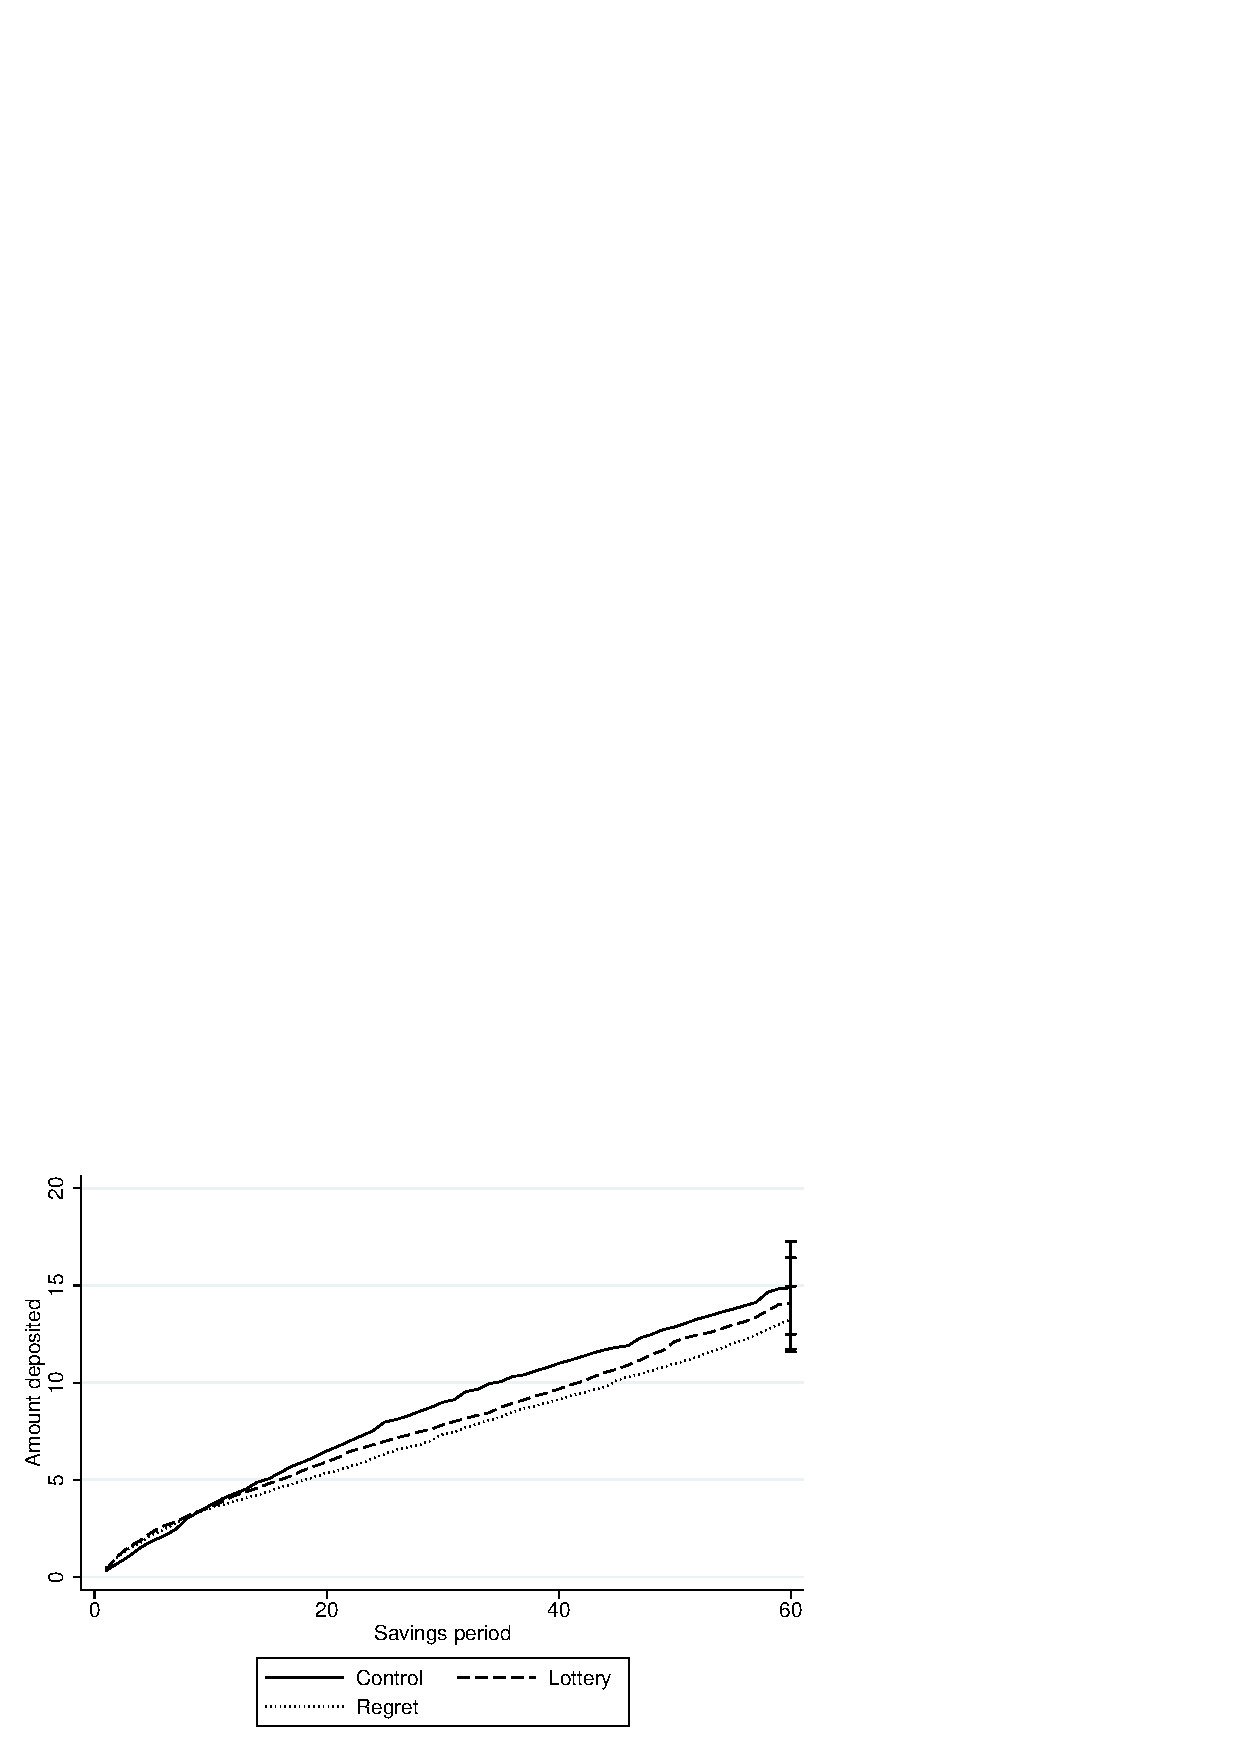
\includegraphics{../../figures/line-cumdepositamount.pdf}
	\end{figure}

	\begin{figure}[!htb]
	\centering
	\caption{No. of deposits made by day t}
	\centerfloat
	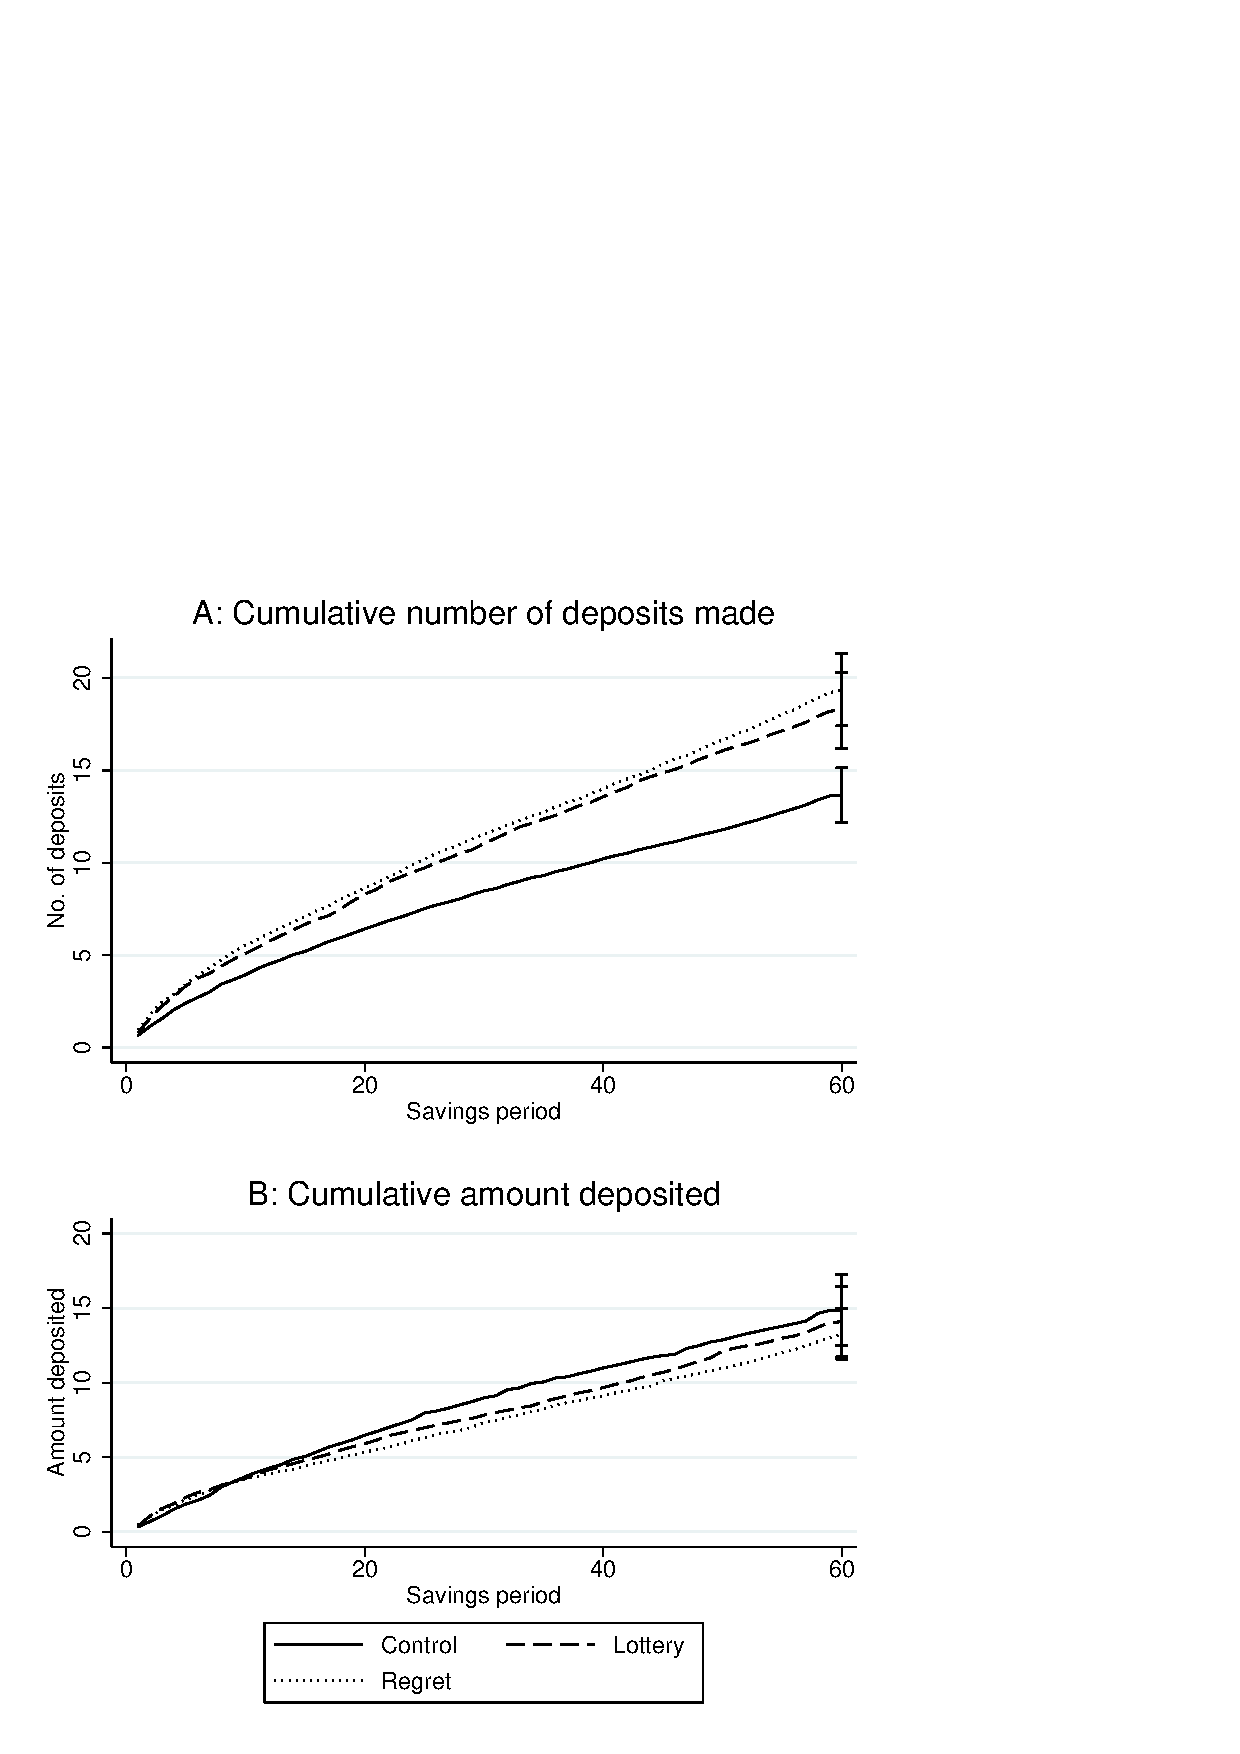
\includegraphics{../../figures/line-cumdeposits.pdf}
	\end{figure}

\clearpage

\bibliographystyle{achicago}
\bibliography{Lottery.bib}

\end{document}